%%%%%%%%%%%%%%%%%%%%%%%%%%%%%%%%%%%%%%%%%%%%%%%%%%%%%%%%%%%%%%%%%%%%%%
% LaTeX Example: Project Report
%
% Source: http://www.howtotex.com
%
% Feel free to distribute this example, but please keep the referral
% to howtotex.com
% Date: March 2011 
% 
%%%%%%%%%%%%%%%%%%%%%%%%%%%%%%%%%%%%%%%%%%%%%%%%%%%%%%%%%%%%%%%%%%%%%%
% How to use writeLaTeX: 
%
% You edit the source code here on the left, and the preview on the
% right shows you the result within a few seconds.
%
% Bookmark this page and share the URL with your co-authors. They can
% edit at the same time!
%
% You can upload figures, bibliographies, custom classes and
% styles using the files menu.
%
% If you're new to LaTeX, the wikibook is a great place to start:
% http://en.wikibooks.org/wiki/LaTeX
%
%%%%%%%%%%%%%%%%%%%%%%%%%%%%%%%%%%%%%%%%%%%%%%%%%%%%%%%%%%%%%%%%%%%%%%
% Edit the title below to update the display in My Documents
%\title{Project Report}
%
%%% Preamble
\documentclass[paper=a4, fontsize=11pt]{scrartcl}
\usepackage[T1]{fontenc}
\usepackage{fourier}
\usepackage{float}
\usepackage[english]{babel}															% English language/hyphenation
\usepackage[protrusion=true,expansion=true]{microtype}	
\usepackage{amsmath,amsfonts,amsthm} % Math packages
\usepackage[pdftex]{graphicx}	
\usepackage{parskip} % Sets space between paragraphs
\usepackage{url}
\usepackage{hyperref}
\usepackage{lineno}
\usepackage{color, soul}
\usepackage{graphicx}
\graphicspath{ {./images/} }

% Adds colours to links
\hypersetup{
    colorlinks=true,
    linkcolor=magenta, % makes links to equations, figs, etc magenta
    urlcolor=blue, % makes url links blue
    citecolor = red % makes citation links red
}

\newcommand{\appropto}{\mathrel{\vcenter{
  \offinterlineskip\halign{\hfil$##$\cr
    \propto\cr\noalign{\kern2pt}\sim\cr\noalign{\kern-2pt}}}}}

%%% Custom sectioning
\usepackage{sectsty}
\allsectionsfont{\centering \normalfont\scshape}


%%% Custom headers/footers (fancyhdr package)
\usepackage{fancyhdr}
\pagestyle{fancyplain}
\fancyhead{}											% No page header
\fancyfoot[L]{}											% Empty 
\fancyfoot[C]{}											% Empty
\fancyfoot[R]{\thepage}									% Pagenumbering
\renewcommand{\headrulewidth}{0pt}			% Remove header underlines
\renewcommand{\footrulewidth}{0pt}				% Remove footer underlines
\setlength{\headheight}{13.6pt}


%%% Equation and float numbering
\numberwithin{equation}{section}		% Equationnumbering: section.eq#
%\numberwithin{figure}{section}			% Figurenumbering: section.fig#
\numberwithin{table}{section}				% Tablenumbering: section.tab#
\usepackage{gensymb}
\usepackage{relsize}
%%% Maketitle metadata
\newcommand{\horrule}[1]{\rule{\linewidth}{#1}} 	% Horizontal rule


%% To use line numbers 
%\linenumbers

%% create a title page
\title{
		%\vspace{-1in} 	
		\usefont{OT1}{bch}{b}{n}
		\normalfont \normalsize \textsc{Queen's University} \\ [25pt]
		\horrule{0.5pt} \\[0.4cm]
		\huge Humpback Whale Identification- Midterm Report \\
		\horrule{2pt} \\[0.5cm]
}
\author{
    \normalfont 
      CISC 867 - Deep Learning Project \\
    \normalfont
    Group Members: \\ 
    \normalsize
    Emily Medema (20340337) \\ 
    \normalsize
    Stephen McKeon (20379475) \\ 
    \normalsize
    Flourish Adebayo (20312488) \\
    October 2022 \\ [3pt]}
\date{\vspace{-5ex}}


%%% Begin document
\usepackage{graphicx}
\graphicspath{ {./images/} }
\begin{document}
%% remove the page number on the title page 
\pagenumbering{gobble}
%% need this line to add the title page you just created 
\maketitle

%% the section command gives a new section with the given header. 


%% go to a new page 
\newpage 
%% start the page numbering again 
\pagenumbering{arabic}

\section*{Introduction}\label{sec: intro}
%Define and motivate the problem, discuss background material or related work, and briefly summarize your approach.
The humpback whale is a species of baleen whale. It has a distinctive body shape with long pectoral fins and a knobbly head. They are known for their infringing and surface behaviour making them popular with whale watchers\cite{kareiva2006whales}. At the beginning of the 20th century, whale populations dropped but increased briefly in the mid-20th century due to the creation of the international whaling committee in 1946\cite{henderson2022behavior}. To better understand the preservation effort, researchers utilize photo surveillance mechanisms to understand marine activities. Various varieties of features of whales such as the shape, tail, markings, and tail length help researchers identify the type of whale they are analyzing \cite{JaisakthiS.M.2017Awms}. In fact, many scientific studies are utilizing photography as a method of monitoring their projects. This usually results in a scientist having to analyze these images themselves, which can take many hours and a lot of technical knowledge \cite{JaisakthiS.M.2017Awms}. However, we can now use image classification models to perform these same tasks in a lot less time with comparable accuracy \cite{JaisakthiS.M.2017Awms}.

Image classification is a booming area of interest in the Computer Vision and Machine Learning fields. Due to the rapid increase of image sharing after the popularity of social media and personal cameras (and later smart phones) \cite{jain2000statistical}, there are a surplus of images to classify and analyze on the internet. There are different algorithms for image classification, the most common of which are deep learning and machine learning. Different models have distinct results in different problem areas, with image classification traditionally using traditional deep learning and machine learning algorithms for its numerous advantages. 

In fact, Deep Neural Networks (DNN) is growing exponentially in the field of Machine Learning (ML). Of the many DNN structures, Convolutional Neural Networks (CNN) are presently the main tool used for image analysis and classification purposes \cite{jain2000statistical}. Comparison and evaluation of images using classification algorithms based on traditional machine learning and deep learning are of great significance for selecting algorithms to classify pictures. 

Different researchers have done various works. In \cite{he2016deep}, Residual Network, commonly referred to as ResNet, was first introduced. It applied residual sections to estimate a denoised image which achieves a classification accuracy comparable to that of a human. In \cite{zhang2006svm}, a SVM KNN was utilized - an improved version of the traditional KNN classifier. It converts the distance of K neighbours and applies a multi-class Support Vector Machine. 

The Humpback Whale Identification Challenge is a Kaggle Competition created to aid whale conservation efforts with the creation of an algorithm to identify individual whales in images. After centuries of intense whaling, recovering whale populations still have a hard time adapting to warming oceans and struggle to compete every day with the industrial fishing industry for food. Scientists use photo surveillance systems to monitor whale activity and can use the shape of whales’ tails and unique markings to identify particular whales and analyze their movements \cite{JaisakthiS.M.2017Awms}.

%% TODO: refined
Data obtained from this challenge were used to compare and analyze popular image classification machine learning models. In this project, we compare a Convolutional Neural Network (CNN) with a CNN augmented with transfer learning, as well as classical machine learning models that detect the identity of humpback whales in the picture.


\subsection{Background}\label{sec: background}

Despite lacking predators, whales have continued to be endangered. As whales play a large role within the oceans ecosystem, conservation efforts have been consistent over the years in order to ensure a stable food chain. Part of these conservation efforts is the tracking of whales to know the health and status of their species by marine biologists. This is mainly done through aerial surveillance and manual identification, which is a very time consuming process \cite{JaisakthiS.M.2017Awms}. As whale fins are identifiable features for individual whales, biologists are able to develop conservation strategies by observing individual whale and entire whale species behaviours. This can take a lot of time and resources. Automating this process with a machine learning model to identify unique whales will alleviate this stress and allow for more time to develop better strategies for the continued survival of whales.

Over the years, a lot of research has been done in this field. There have been multiple Kaggle competitions and there are a multitude of approaches to this problem. While there have been some studies on the application of transfer learning augmenting deep learning and classical machine learning models \cite{YuanHongchun2020AAIC}, it's effectiveness in this particular problem space compared to a classical machine learning model, such as SVM, as well as a deep learning model itself (without transfer learning) can be further explored.

\section{Data}\label{sec: data}

The \href{https://www.kaggle.com/competitions/humpback-whale-identification/overview}{Humpback Whale Identification} competition on Kaggle contains thousands of images of humpback whale flukes - 25,361 files for training and a further 7,960 for testing. Individual whales have been identified by researchers and given an identification (Id). The challenge is to predict the whale Id of images in the test set. This is particularly challenging for two primary reasons:
\begin{itemize}
  \item The heterogeneity of the data. Images drastically vary in size. Some are greyscale, others are in colour. Some whale flukes are pointing towards the sky, others are not. Normalizing the data will be extremely important and is discussed in \autoref{subsec:Preprocessing}.
  \item Imbalance in the dataset. There is a relatively small dataset compared to the 5,000 unique whale Ids present in the data. Only 227 whales are represented in the dataset more than 10 times while over 2,000 whales are represented by only a single sample, as shown in \autoref{fig:ID_Occ}. To compensate for this we will be utilizing data augmentation as discussed later in \autoref{subsec:Augmentation}.
\end{itemize}

%This isn't a great image, there's too much info in its current form to really be legible. For now, it gets the point across.
\begin{figure}[H]
    \caption{Number of samples per unique whale Id}
    \centering
    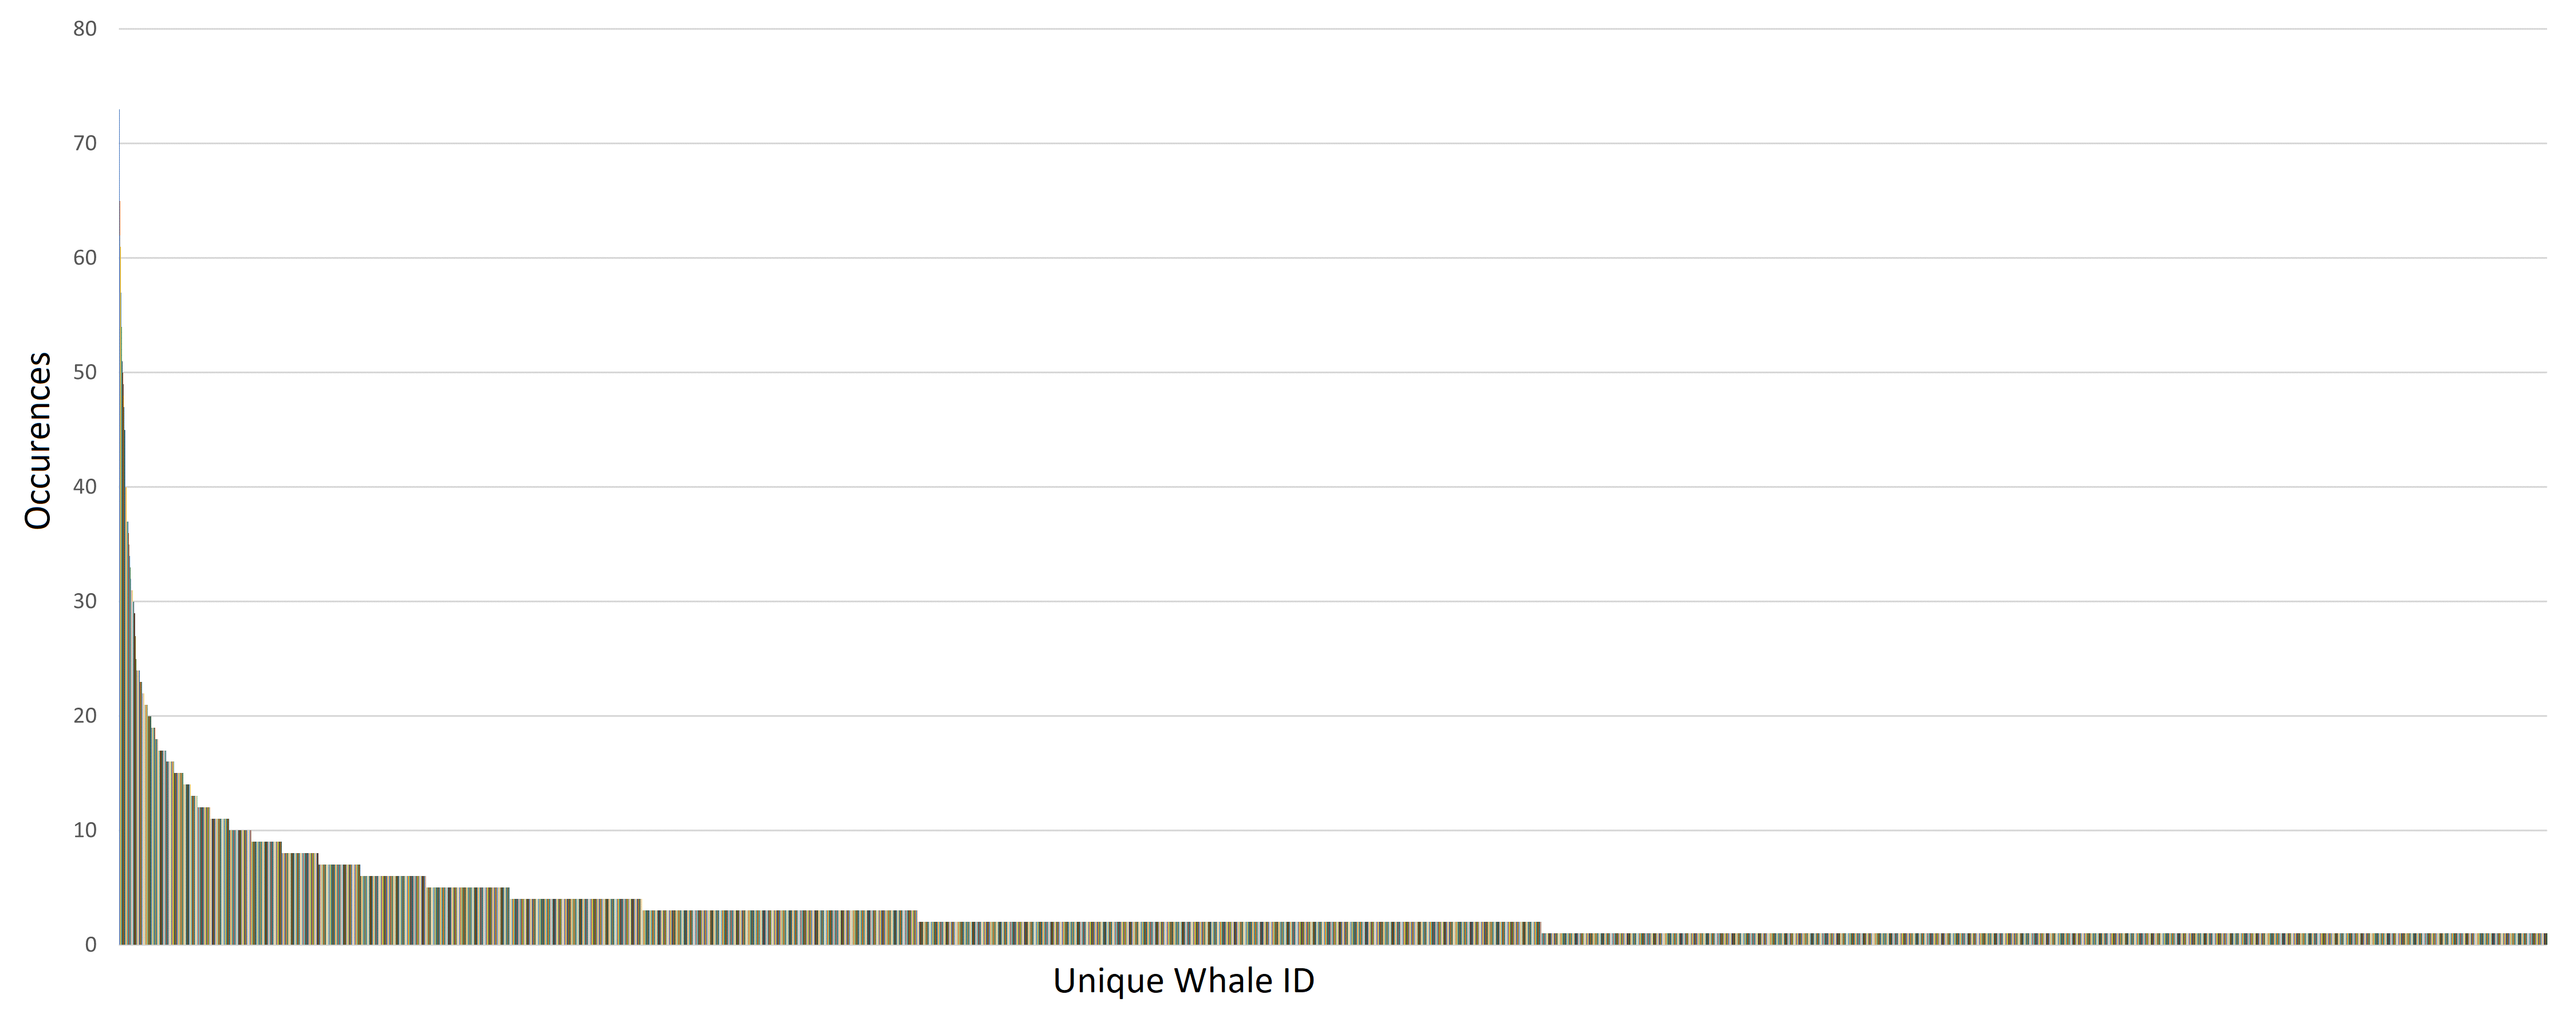
\includegraphics[width=\textwidth]{ID_Occurences.png}
    \label{fig:ID_Occ}
\end{figure}

\section{Methodology}\label{sec: meth}

%Details of the approach: Include any formulas, pseudocode, diagrams -- anything that is necessary to clearly explain your system and what you have done. If possible, illustrate the intermediate stages of your approach with results images.

%TODO: finish the machine learning model section

To identify whales by their fluke data preprocessing would be conducted to remove noise and crop to show only the fluke. Due to the sparse number of images of the same whale, we will perform data augmentation by flipping and rotating the underrepresented whale Id images. This will allow us to develop a more accurate and robust model. We will then attempt to identify the whale via a developed CNN model, a CNN augmented with transfer learning, and a SVM.

The steps involved in this identifying system are:
\begin{itemize}
    \item Preprocessing the data
    \item Augmentation of the data
    \item Classification with CNN
    \item Classification with CNN augmented with transfer learning
    \item Classification with SVM
    \item Comparison of Results
\end{itemize}

\subsection{Data Preprocessing}\label{subsec:Preprocessing}

The first step for the processing of the data was to crop as much noise from the images as possible, such as the background in the images. While many of the whale pictures in the dataset were already cropped tightly around the whale fluke, in some images the whale fluke occupied only a small area of the picture. Zooming onto the relevant part of the picture provides greater accuracy to a classification model. 

A couple of months before this competition, a playground version of the same competition was hosted on Kaggle, but, as it was noted by the competition hosts, the real version featured even more data and cleaner labels. We were able to leverage the pre-trained weights from a CNN model from the playground version of the competition that identified the coordinates specifying a bounding box around the fluke of the whale in each image.The CNN model used to determine the proper bounding box of the whale fluke in each image was quite complex, as shown in \autoref{tab:table1}. Leveraging the weights from the trained model saved a lot of time.

\begin{table}[h!]
  \begin{center}
    \caption{CNN - Bounding Box Model}
    \label{tab:table1}
    \begin{tabular}{l|c|r} % <-- Alignments: 1st column left, 2nd middle and 3rd right, with vertical lines in between
      \textbf{Layer} & \textbf{Output Shape} & \textbf{Params}\\
      \hline
      InputLayer & (128, 128, 1) & 0\\
      Conv2D & (128, 128, 64) & 5248\\
      Conv2D & (128, 128, 64) & 36928\\
      BatchNormalization & (128, 128, 64) & 256\\
      Conv2D & (64, 64, 64) & 16448\\
      Conv2D & (64, 64, 64) & 36928\\
      Conv2D & (64, 64, 64) & 36928\\
      BatchNormalization & (64, 64, 64) & 256\\
      Conv2D & (32, 32, 64) & 16448\\
      Conv2D & (32, 32, 64) & 36928\\
      Conv2D & (32, 32, 64) & 36928\\
      BatchNormalization & (32, 32, 64) & 256\\
      Conv2D & (16, 16, 64) & 16448\\
      Conv2D & (16, 16, 64) & 36928\\
      Conv2D & (16, 16, 64) & 36928\\
      BatchNormalization & (16, 16, 64) & 256\\
      Conv2D & (8, 8, 64) & 16448\\
      Conv2D & (8, 8, 64) & 36928\\
      Conv2D & (8, 8, 64) & 36928\\
      BatchNormalization & (8, 8, 64) & 256\\
      Conv2D & (4, 4, 64) & 16448\\
      Conv2D & (4, 4, 64) & 36928\\
      Conv2D & (4, 4, 64) & 36928\\
      BatchNormalization & (4, 4, 64) & 256\\
      MaxPooling2D\_1 & (4, 1, 64) & 0\\
      MaxPooling2D\_2 & (1, 4, 64) & 0\\
      Flatten\_1 & (256) & 0\\
      Flatten\_2 & (256) & 0\\
      Dense\_1 & (16) & 4112\\
      Dense\_2 & (16) & 4112\\
      Concatenate & (32) & 0\\
      Dense & (4) & 132\\
    \end{tabular}
      \small
      \item Trainable params: 502,820
  \end{center}
\end{table}

By describing the same neural network and loading the pre-trained weights, the training dataset could then be passed to the model and evaluated to obtain the coordinates for bounding boxes around the whales' flukes. These coordinates can then be used to visualize the bounding box region, as shown in \autoref{fig:fig1}.

\begin{figure}[h]
    \caption{Coordinates for Bounding Box overlayed on the corresponding images}
    \centering
    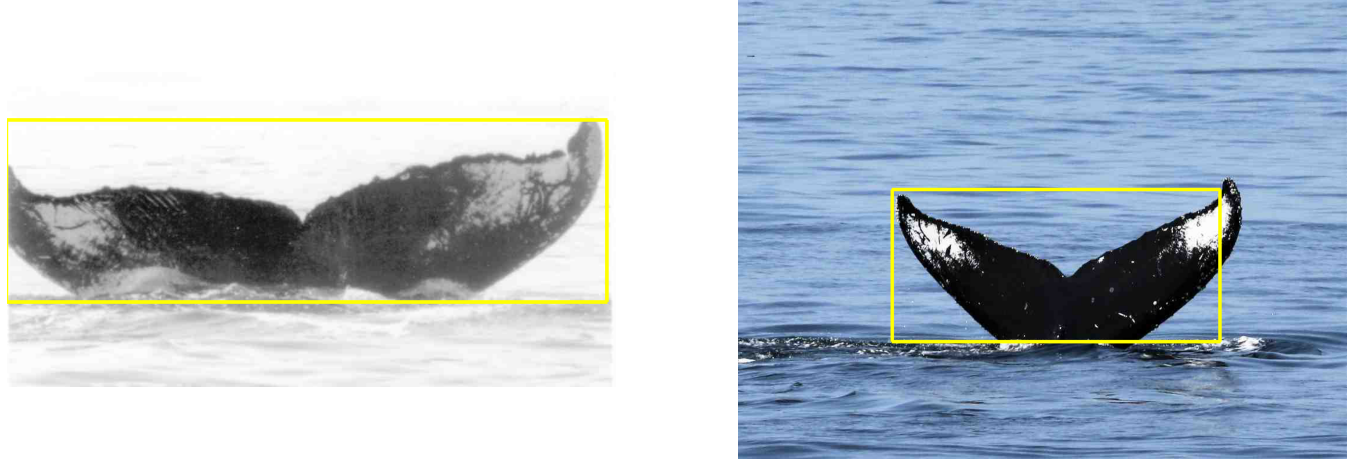
\includegraphics[width=0.5\textwidth]{BoundingBoxExample.png}
    \label{fig:fig1}
\end{figure}

\begin{figure}[h]
    \caption{Original images (left) and their corresponding processed images (right)}
    \centering
    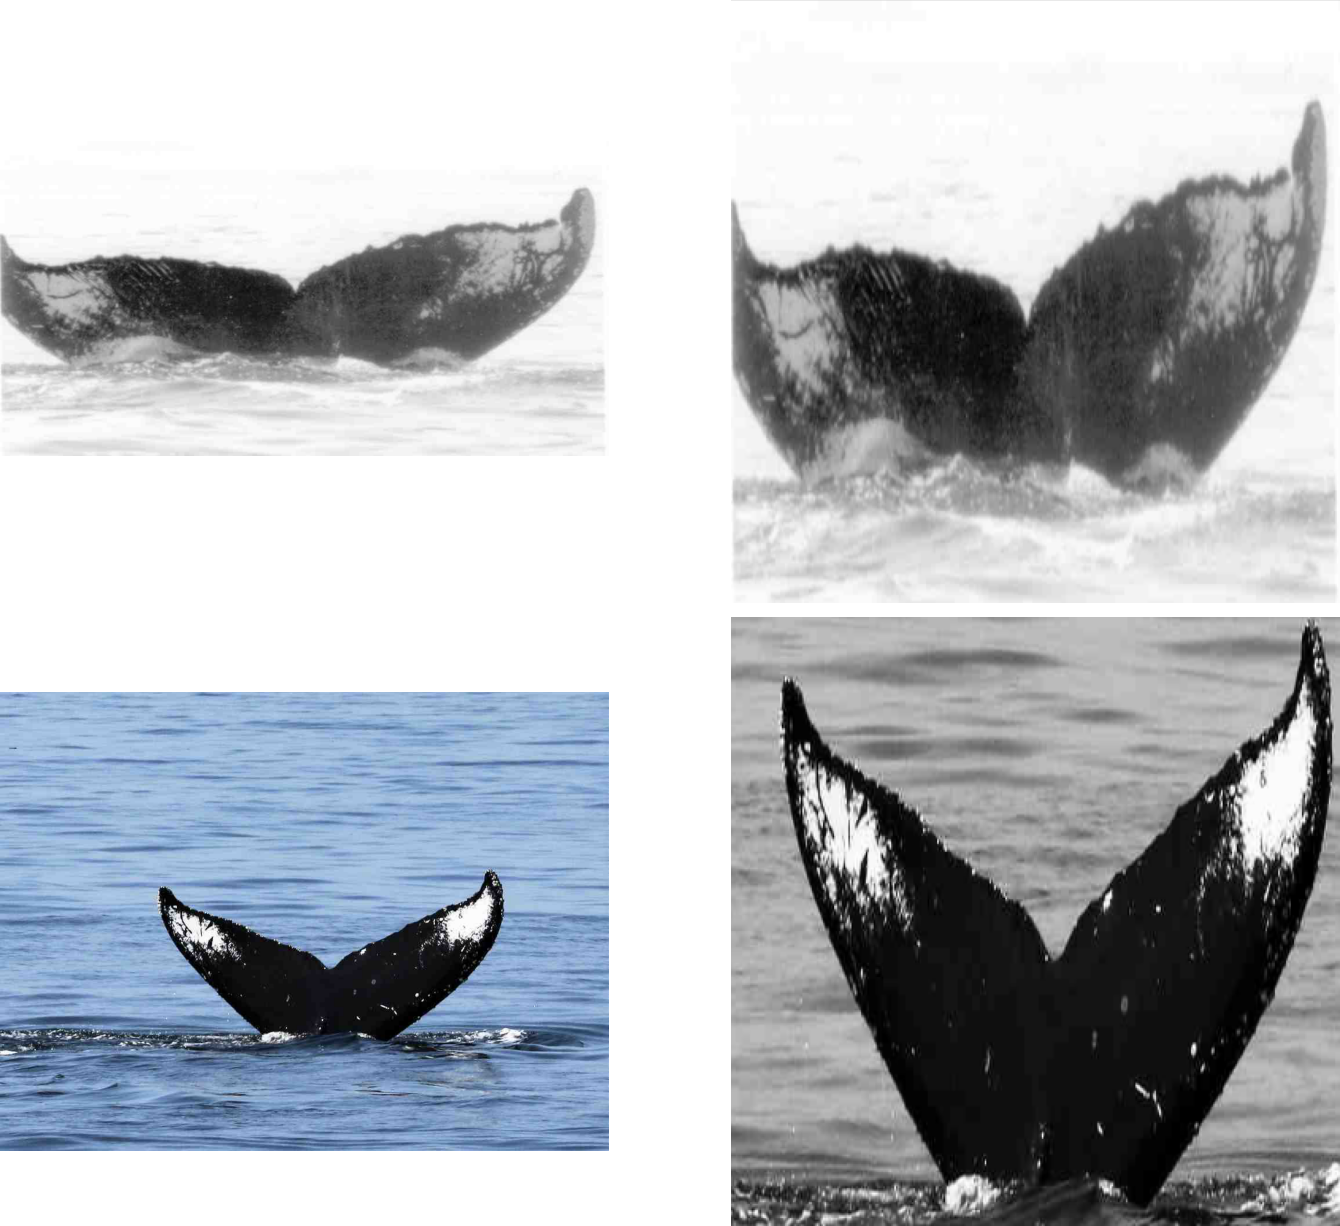
\includegraphics[width=0.5\textwidth]{ProcessedImages.png}
    \label{fig:fig2}
\end{figure}

As you can see, the resulting bounding boxes are not perfect. This can be resolved by extending the region described by the bounding box before cropping the image. The idea is that clipping the edges of the fluke is more harmful than the noise obtained by fitting it exactly, thus an increased margin is preferred. Through trial and error, we determined that extending the crop region by 8\% was sufficient to ensure the entire fluke was captured. This is shown to have succeeded when comparing the coloured image from \autoref{fig:fig1} with the output from \autoref{fig:fig2}.

As shown in the previous \autoref{fig:fig1}, some of the images in the dataset are greyscale and some are colour. In order to standardize the data and ensure our model does not learn any colour-only or greyscale-only specific features, we converted all images to greyscale.

An affine transformation is a geometric transformation that preserves lines and parallelism - but not necessarily distances and angles. The final step for data preprocessing was to take the cropped area from the previous step and transform it to a uniform size for use as input to a neural network - in our case, 384x384x1 (only one channel for black and white). The resulting changes after cropping, converting to greyscale, and applying the affine transformation to the images from the previous figure are shown in \autoref{fig:fig2}. With these changes, the data is normalized so that there is as little variation as possible within the dataset aside from the differences between each whale's flukes.

One final manipulation of the data was the removal of particular samples. In the training dataset, numerous samples were classified as "new\_whale" as opposed to the identification number associated with a particular individual whale. The image features associated with the various "new\_whale" samples, however, do not share any logical overlap. They are different individuals. While these samples would be useful in the testing phase of our model, they do not contribute to proper learning during training; hence, they were removed.

\subsection{Data Augmentation}\label{subsec:Augmentation}
Due to the nature of the data - that is, certain classes with numerous instances and many classes with only one instance - we will have to heavily augment the data. The intent is to augment the data by a combination of flipping and rotating, with perhaps Gaussian noise, random crops, and random blur as well. The intent is to put an emphasis on creating more samples for classes that are under represented, so these will be augmented with every possible combination of our augmentation strategies, while over represented classes will remain untouched. 

\subsection{Model Training}

The first model we will utilize for classification is a CNN using the python library Keras. Before we could train the model itself, we had to transform the data into a form that could be utilized for classification, as discussed in  \autoref{subsec:Preprocessing}. After reading in the data, we separated the X and Y (i.e., input and output variables), the image name and the whale id respectively. We then read in the images for each image name as an array. We then hot-encoded our response variable which will help with classifying the output of the CNN. Once the transformation of the data was done, we began to build our model.

We decided to set the padding of the model to "same" and the activation function to "relu" throughout. Similarly, we decided to utilize max-pooling. In essence, this means our output shape follows the following equation: $output\_shape = math.floor((input_shape - 1) / strides) + 1$. We also used BatchNormalization and Dropout in order to prevent over-fitting. The Adam optimizer was used to optimize the gradient descent of our model.

In order to determine if this model architecture will work for our data, we train it with 10\% of the training data. If the model overfits onto this subset of the data, that means the model will most likely accurately work on the entire dataset.

After running the model on the subset of data, we received an overfitting of the data as seen in Figure \ref{fig:cnn_acc_10p} and Figure \ref{fig:cnn_loss_10p} with extremely high accuracy and extremely low loss.

\begin{figure}[h]
    \centering
    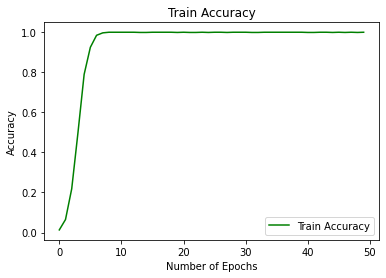
\includegraphics[width=0.5\textwidth]{training_cnn_acc_10p.png}
    \caption{Training Accuracy on 10\% of Training Data}
    \label{fig:cnn_acc_10p}
\end{figure}

\begin{figure}[h]
    \centering
    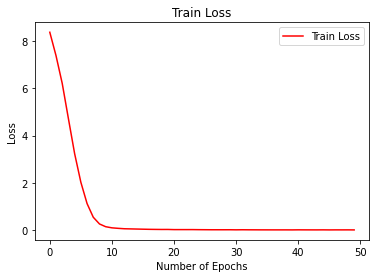
\includegraphics[width=0.5\textwidth]{training_10p_loss.png}
    \caption{Training Loss on 10\% of Training Data}
    \label{fig:cnn_loss_10p}
\end{figure}

\subsubsection{Hyperparameter Tuning}

[Under Construction]

\subsection{Model Testing}

[Under Construction]

\section{Experiment}\label{sec: experiment}

[Under Construction]

\section{Conclusion}\label{sec: conlusion}

[Under Construction]
 
\clearpage
\bibliography{references} 
\bibliographystyle{ieeetr}



%%% End document
\end{document}